%!TEX root = mainfile.tex

\section{Introduction} % (fold)
\label{sec:introduction}
	Tomography is a technique for imaging objects and examining the internal structure of them in a non-invasive way. It is of enormous use in the medical industry where the ability to view the inside of a patient's body can be invaluable in the diagnostic process. Tomography stands out from other methods of viewing the internal structures of objects since it is able to view a slice through the object without the addition of the material around it in other slices, i.e.\ the rest of the object does not obscure the slice being viewed.

    Tomography can be applied to many different imaging techniques, x-ray, MRI and ultrasound, and has been applied to many areas of scientific study and research including medicine, chemistry, astronomy and geology.

    Tomographic reconstruction involves the creation of an image of an object taken through a particular slice by recombining the data collected from a set of line integrals across that object in the plane of interest. In other words, it is the conversion of a 3D averaged, or integrated, view of an object into a 2D slice of the object at a particular location, so that the details of the interior can be examined.

    The word tomography comes from the Greek \textit{tomos} meaning section and \textit{graphein} meaning to write, so tomography is simply writing `parts' of an object, in this case an image of a single plane through that object, in a useful form.
% section introduction (end)

\section{Tomographic Reconstruction} % (fold)
\label{sec:tomographic_reconstruction}
    In order to examine this method of image construction, we shall use a series of images which form \textit{sagittal} slices of a human head. This means that each of the 129 images in the collection are a slice from side to side at a slightly different position. Together, they form a 3 dimensional image of the head, with all of the interior detail maintained. A few of these images are shown in figure~\ref{fig:example_sagittal}
    \begin{figure}[ht]
        \centering
        \begin{minipage}[c]{0.19\linewidth}
            \centering
            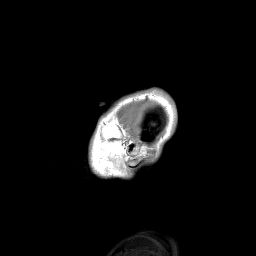
\includegraphics[width=\textwidth]{Files/report_images/sagittal_example1.jpg}
        \end{minipage}
        \begin{minipage}[c]{0.19\linewidth}
            \centering
            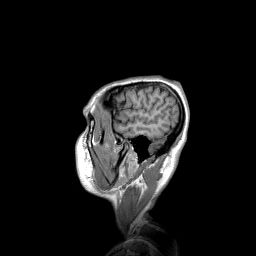
\includegraphics[width=\textwidth]{Files/report_images/sagittal_example2.jpg}
        \end{minipage}
        \begin{minipage}[c]{0.19\linewidth}
            \centering
            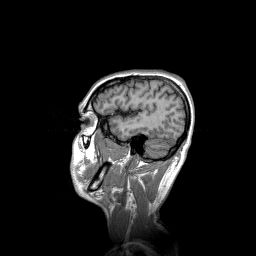
\includegraphics[width=\textwidth]{Files/report_images/sagittal_example3.jpg}
        \end{minipage}
        \begin{minipage}[c]{0.19\linewidth}
            \centering
            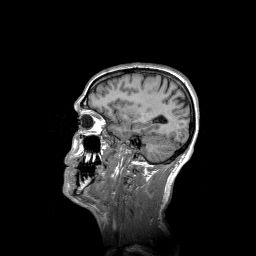
\includegraphics[width=\textwidth]{Files/report_images/sagittal_example4.jpg}
        \end{minipage}
        \begin{minipage}[c]{0.19\linewidth}
            \centering
            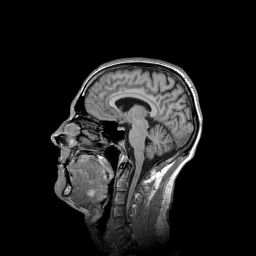
\includegraphics[width=\textwidth]{Files/report_images/sagittal_example5.jpg}
        \end{minipage}
        \caption{Example slices from the original sagittal 3D image that will be used to examine the tomographic reconstruction method. Out of the 129 images that make up the full image, these are, from left to right, image 20, 31. 38, 48 and 64 respectively.\label{fig:example_sagittal}}
    \end{figure}

    In order to demonstrate the tomographic reconstruction method as used in medical applications, an effective CT scan can be taken of this 3D image by converting it to axial slices. These are slices taken laterally through the object from top to bottom. Again, a selection of this new 3D image is shown in figure~\ref{fig:example_axial}.
    \begin{figure}[ht]
        \centering
        \begin{minipage}[c]{0.3\linewidth}
            \centering
            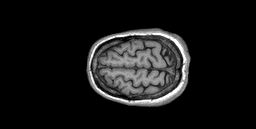
\includegraphics[width=\textwidth]{Files/report_images/axial_example1.jpg}
        \end{minipage}
        \begin{minipage}[c]{0.3\linewidth}
            \centering
            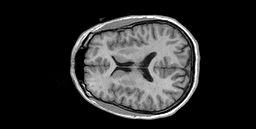
\includegraphics[width=\textwidth]{Files/report_images/axial_example2.jpg}
        \end{minipage}
        \begin{minipage}[c]{0.3\linewidth}
            \centering
            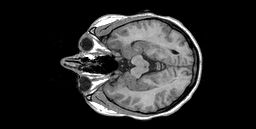
\includegraphics[width=\textwidth]{Files/report_images/axial_example3.jpg}
        \end{minipage}

        \begin{minipage}[c]{0.3\linewidth}
            \centering
            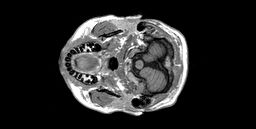
\includegraphics[width=\textwidth]{Files/report_images/axial_example4.jpg}
        \end{minipage}
        \begin{minipage}[c]{0.3\linewidth}
            \centering
            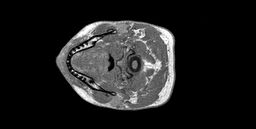
\includegraphics[width=\textwidth]{Files/report_images/axial_example5.jpg}
        \end{minipage}
        \begin{minipage}[c]{0.3\linewidth}
            \centering
            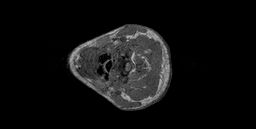
\includegraphics[width=\textwidth]{Files/report_images/axial_example6.jpg}
        \end{minipage}
        \caption{Example slices from the original sagittal 3D image that will be used to examine the tomographic reconstruction method. Out of the 129 images that make up the full image, these are, from top left to bottom right, image 78, 106, 126, 162 and 182 respectively.\label{fig:example_axial}}
    \end{figure}

    In order to show the effectiveness of the different techniques used in tomographic reconstruction, we shall refer back to a single of these slices, which will be the one that shall be reconstructed. This reference image will be image NUM out of the 256 stack above, and is shown in figure~\ref{fig:reference_slice}.
    \begin{figure}[ht]
        \centering
        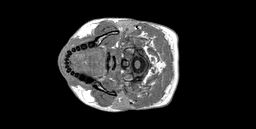
\includegraphics[width=0.4\textwidth]{Files/report_images/reference_slice.jpg}
        \caption{Reference slice that shall be used to compare later.\label{fig:reference_slice}}
    \end{figure}

    \subsection{Tomographic Scanner} % (fold)
    \label{sub:tomographic_scanner}
        When used in medical imaging applications, the data that is collected by a tomographic scanner would be represented by the image in figure~\ref{fig:3d_scan_example}.
        \begin{figure}[ht]
            \centering
                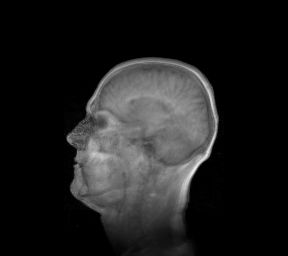
\includegraphics[width=0.4\textwidth]{Files/report_images/3D_scan_example.jpg}
            \caption{An image of the 3 dimensional representation of an object that would be measured by a tomographic scanner. This is just one view of the $360^{\circ}$ image that is generated.\label{fig:3d_scan_example}}
        \end{figure}

        The full image consists of a number of views of the object, each showing what it looks like from a different angle, averaged or integrated over its depth. Tomographic reconstruction involves calculating the reference image above, starting from this 3D representation
    % subsection tomographic_scanner (end)
% section tomographic_reconstruction (end)

\section{Back Projection} % (fold)
\label{sec:back_projection}
    The general method for tomographic reconstruction is called back projection. There are number of variations on this method that provide varying quality of results. We shall first examine the basic method of back projection and then see how it can be improved to increase the accuracy of the images calculated with it.

    \subsection{Sinogram} % (fold)
    \label{sub:sinogram}
        Since we now have a 3D image, such as would be collected when imaging an object from a large number of different angles around it, we can no longer determine what the interior contains. The first step to finding this is the plot a sinogram. Each slide of the 3D image is a view of the object from a particular angle. Since we require to see the interior of the object only through a particular single slice, most of the 3D image is not needed. Thus the useful information is a series of single pixel tall images of a single slice of the object taken at slightly different angle around it.

        A sinogram is a combined image of all of these views plotted as the value of the line integral with $x'$ against the angle $theta$, as per the diagram in figure~\ref{fig:sinogram_diag}. Since the different views are all taken about a single static point, polar co-ordinates are used, such that
        \begin{align}
            x\cos(\theta) + y\sin(\theta) = x'
        \end{align}
        Thus, the set of measurements that are collected for a given angle, $\theta$, make up a single layer of figure~\ref{fig:example_sinogram} and are called the parallel projection of the object at the angle $\theta$, denoted as $P_{\theta}(x')$.
        \begin{figure}[ht]
            \begin{center}
                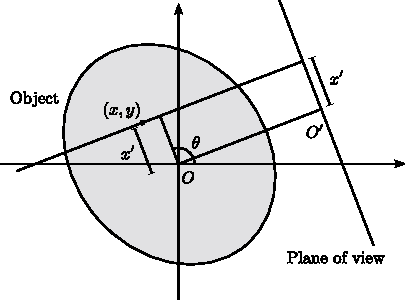
\includegraphics[width=0.5\textwidth]{Files/report_images/sinogram_diag.pdf}
            \end{center}
            \caption{A sinogram is an image of the value of the line integral plotted against angle for all the views around a measured object. Each point from the object traces a sinusoidal line as the angle is increased, or as the object is rotated in front of the measuring device.\label{fig:sinogram_diag}}
        \end{figure}

        An example of a sinogram, showing the plot for the data concerning the slice that holds the information for the reference image above, is shown in figure~\ref{fig:example_sinogram}.
        \begin{figure}[ht]
            \begin{center}
                
\includegraphics[width=0.4\textwidth]{Files/report_images/example_sinograph.jpg}
            \end{center}
            \caption{A sinogram is an image of the value of the line integral plotted against angle for all the views around a measured object. Each point from the object traces a sinusoidal line as the angle is increased, or as the object is rotated in front of the measuring device.\label{fig:example_sinogram}}
        \end{figure}


    % subsection sinogram (end)
% section back_projection (end)

